% =============================================================================
%  S&P 500 Price Movement Prediction --- FPA Final Presentation
%  Tecnologico de Monterrey, M.Sc. in Computer Science --- Data Analytics
%  Authors: Cesar Emilio Castano Marin (A00830006)
%           Brenda Angelica Garcia    (A01633622)
%  Compile with: pdflatex (Overleaf-compatible)
% =============================================================================
\documentclass[aspectratio=169,11pt]{beamer}

% ---------- Encoding & fonts ----------
\usepackage[T1]{fontenc}
\usepackage[utf8]{inputenc}
\usepackage{lmodern}
\usepackage[default,scale=0.95]{opensans}
\renewcommand{\familydefault}{\sfdefault}

% ---------- Core packages ----------
\usepackage{graphicx}
\usepackage{booktabs}
\usepackage{array}
\usepackage{tabularx}
\usepackage{amsmath,amssymb}
\usepackage{tikz}
\usepackage{xcolor}
\usepackage{calc}
\usepackage{appendixnumberbeamer}
\usetikzlibrary{positioning,shapes.geometric,arrows.meta,fit,backgrounds}

% ---------- Colour palette (Tec de Monterrey inspired) ----------
\definecolor{TecBlue}{HTML}{0F3D60}      % deep institutional blue
\definecolor{TecBlueDark}{HTML}{082842}  % darker accent
\definecolor{TecGold}{HTML}{C8A951}      % warm gold accent
\definecolor{TecGray}{HTML}{4A4A4A}      % body text
\definecolor{TecLight}{HTML}{F4F6F9}     % background highlight
\definecolor{TecGreen}{HTML}{1B7A4B}     % positive deltas
\definecolor{TecRed}{HTML}{B23A48}       % negative deltas

% ---------- Beamer theme ----------
\usetheme{default}
\usecolortheme{default}
\useinnertheme{default}
\useoutertheme{infolines}
\setbeamertemplate{navigation symbols}{}
\setbeamertemplate{itemize items}[circle]
\setbeamertemplate{itemize subitem}[triangle]
\setbeamertemplate{enumerate items}[default]
\setbeamercolor{normal text}{fg=TecGray}
\setbeamercolor{structure}{fg=TecBlue}
\setbeamercolor{frametitle}{fg=white,bg=TecBlue}
\setbeamercolor{title}{fg=TecBlue}
\setbeamercolor{subtitle}{fg=TecGold}
\setbeamercolor{author}{fg=TecGray}
\setbeamercolor{date}{fg=TecGray}
\setbeamercolor{block title}{fg=white,bg=TecBlue}
\setbeamercolor{block body}{bg=TecLight,fg=TecGray}
\setbeamercolor{alerted text}{fg=TecGold}
\setbeamercolor{section in toc}{fg=TecBlue}
\setbeamercolor{subsection in toc}{fg=TecGray}

% ---------- Typography ----------
\setbeamerfont{title}{size=\Large,series=\bfseries}
\setbeamerfont{subtitle}{size=\normalsize,series=\mdseries}
\setbeamerfont{frametitle}{size=\large,series=\bfseries}
\setbeamerfont{block title}{size=\small,series=\bfseries}

% ---------- Frame title template ----------
\setbeamertemplate{frametitle}{%
  \nointerlineskip
  \begin{beamercolorbox}[wd=\paperwidth,ht=2.6ex,dp=1.4ex,leftskip=0.9cm,rightskip=0.9cm]{frametitle}%
    \strut\insertframetitle\strut
  \end{beamercolorbox}%
  \vskip-2pt
  \begin{tikzpicture}[remember picture,overlay]
    \fill[TecGold] (current page.north west) ++(0,-1.05cm) rectangle ++(\paperwidth,-1pt);
  \end{tikzpicture}%
}

% ---------- Footline ----------
\setbeamertemplate{footline}{%
  \leavevmode%
  \hbox{%
    \begin{beamercolorbox}[wd=.45\paperwidth,ht=2.25ex,dp=1ex,leftskip=0.9cm]{author in head/foot}%
      \usebeamerfont{author in head/foot}\color{TecGray}\scriptsize C.~Castano \& B.~Garcia
    \end{beamercolorbox}%
    \begin{beamercolorbox}[wd=.45\paperwidth,ht=2.25ex,dp=1ex,center]{title in head/foot}%
      \usebeamerfont{title in head/foot}\color{TecGray}\scriptsize S\&P 500 Direction Prediction --- FPA
    \end{beamercolorbox}%
    \begin{beamercolorbox}[wd=.10\paperwidth,ht=2.25ex,dp=1ex,rightskip=0.9cm,right]{date in head/foot}%
      \usebeamerfont{date in head/foot}\color{TecGray}\scriptsize \insertframenumber/\inserttotalframenumber
    \end{beamercolorbox}}%
  \vskip0pt%
}

% ---------- Margins on body content ----------
\setbeamersize{text margin left=0.9cm,text margin right=0.9cm}

% ---------- Custom commands ----------
\newcommand{\good}[1]{{\color{TecGreen}\textbf{#1}}}
\newcommand{\bad}[1]{{\color{TecRed}\textbf{#1}}}
\newcommand{\heading}[1]{{\color{TecBlue}\textbf{#1}}}

\graphicspath{{figures/}}

% =============================================================================
%  Title metadata
% =============================================================================
\title[S\&P 500 Direction Prediction]{S\&P 500 Stock Price Movement Prediction}
\subtitle{Historical Market Data and Financial News Sentiment Analysis}
\author[C. Castano \& B. Garcia]{%
  C\'esar Emilio Casta\~no Mar\'in \textsuperscript{A00830006} \\
  Brenda Ang\'elica Garc\'ia \textsuperscript{A01633622}}
\institute{School of Engineering and Sciences \\ Tecnol\'ogico de Monterrey \\ \textit{M.Sc. in Computer Science --- Data Analytics}}
\date{Final Project Presentation --- May 2026}

% =============================================================================
\begin{document}

% ------------------------------ Title page -----------------------------------
{
\setbeamertemplate{footline}{}
\begin{frame}[plain]
\begin{tikzpicture}[remember picture,overlay]
  \fill[TecBlue]    (current page.north west) rectangle ([yshift=-2cm]current page.north east);
  \fill[TecGold]    ([yshift=-2cm]current page.north west) rectangle ([yshift=-2.08cm]current page.north east);
  \fill[TecBlueDark] (current page.south west) rectangle ([yshift=1.2cm]current page.south east);

  \node[anchor=north west,white,inner sep=0pt] at ([xshift=0.9cm,yshift=-0.55cm]current page.north west)
    {\scriptsize\textbf{TECNOL\'OGICO DE MONTERREY}~$\cdot$~SCHOOL OF ENGINEERING AND SCIENCES};
  \node[anchor=north east,white,inner sep=0pt] at ([xshift=-0.9cm,yshift=-0.55cm]current page.north east)
    {\scriptsize\textbf{Data Analytics --- Final Project}};

  \node[anchor=west,white,text width=14cm,inner sep=0pt] at ([xshift=0.9cm,yshift=0.4cm]current page.center)
    {\fontsize{22}{26}\selectfont\textbf{S\&P 500 Stock Price Movement Prediction}\\[4pt]
     \fontsize{14}{18}\selectfont\textit{Historical Market Data and Financial News Sentiment Analysis}};

  \node[anchor=west,TecGray,text width=14cm,inner sep=0pt] at ([xshift=0.9cm,yshift=-1.45cm]current page.center)
    {\fontsize{11}{14}\selectfont
     \textbf{C\'esar Emilio Casta\~no Mar\'in} \,\textcolor{TecGold}{$\bullet$}\, A00830006 \\[2pt]
     \textbf{Brenda Ang\'elica Garc\'ia}     \,\textcolor{TecGold}{$\bullet$}\, A01633622 \\[10pt]
     \textit{M.Sc. in Computer Science --- Semester 4}};

  \node[anchor=south west,white,inner sep=0pt] at ([xshift=0.9cm,yshift=0.4cm]current page.south west)
    {\scriptsize Final Project Presentation};
  \node[anchor=south east,white,inner sep=0pt] at ([xshift=-0.9cm,yshift=0.4cm]current page.south east)
    {\scriptsize May 2026};
\end{tikzpicture}
\end{frame}
}

% ------------------------------ Agenda ---------------------------------------
\begin{frame}{Agenda}
\vspace{2pt}
\begin{columns}[T,onlytextwidth]
  \column{0.5\textwidth}
  \begin{enumerate}
    \item Motivation \& research framing
    \item Hypotheses and research questions
    \item Related work
    \item End-to-end methodology
    \item Datasets and feature engineering
  \end{enumerate}
  \column{0.5\textwidth}
  \begin{enumerate}\setcounter{enumi}{5}
    \item Sentiment pipeline (FinBERT)
    \item Experimental design
    \item Results --- technical only
    \item Results --- technical + sentiment
    \item Discussion, limitations \& conclusions
  \end{enumerate}
\end{columns}
\end{frame}

% ------------------------------ Motivation -----------------------------------
\begin{frame}{Motivation}
\begin{columns}[T,onlytextwidth]
\column{0.58\textwidth}
\begin{itemize}
  \item The \heading{S\&P 500} is the most-watched benchmark of U.S. equity market health, with eleven GICS sectors that behave very differently in volatility and news flow.
  \item Predicting next-day price \heading{direction} (not price) has direct value for risk management and tactical allocation.
  \item Markets are not perfectly efficient: behavioural biases, herd behaviour, and delayed information assimilation create exploitable signals.
  \item Recent NLP advances (FinBERT) make it cheap to extract structured sentiment from financial text.
\end{itemize}

\column{0.40\textwidth}
\begin{block}{Research question}
Does a tree-based ensemble of technical indicators \alert{plus} short-form news sentiment beat a technical-only baseline at predicting the next-day direction of the S\&P 500 --- and does the gain grow with sector volatility?
\end{block}
\end{columns}
\end{frame}

% ------------------------------ Problem framing ------------------------------
\begin{frame}{Problem statement and hypotheses}
\begin{block}{Binary classification target}
\centering\small
$y_t = \begin{cases} 1 & \text{if } C_{t+1} > C_t \text{ (upward)} \\ 0 & \text{if } C_{t+1} \leq C_t \text{ (no change or downward)} \end{cases}$
\end{block}

\begin{columns}[T,onlytextwidth]
\column{0.5\textwidth}
\heading{H1.} Adding FinBERT-derived sentiment to a technical-only baseline \textit{improves} Accuracy, F1, and AUC-ROC.

\vspace{6pt}
\heading{H2.} The sentiment gain is \textit{larger} for sectors with higher historical volatility.

\column{0.5\textwidth}
\heading{Research questions}
\begin{enumerate}
  \item Does sentiment improve daily direction prediction?
  \item Random Forest or XGBoost --- which wins?
  \item Does sector volatility modulate the sentiment benefit?
\end{enumerate}
\end{columns}

\vspace{6pt}
\small \textbf{Note.} We predict \textit{trend}, not exact prices. Flat days ($C_{t+1}=C_t$) are grouped with class~0 because they do not represent an upward trend; for liquid indices these days are rare.
\end{frame}

% ------------------------------ Related Work ---------------------------------
\begin{frame}{Related work --- five anchor references}
\small
\begin{itemize}
  \item \heading{Bollen et al. (2011)} --- Twitter mood predicts DJIA direction with 87.6\% accuracy. \textit{Sentiment carries predictive information beyond price.}
  \item \heading{Vargas et al. (2017)} --- CNN/RNN on Reuters news + technicals beats single-modality baselines. \textit{Multimodal helps, but is compute heavy.}
  \item \heading{Araci (2019)} --- FinBERT, BERT fine-tuned on financial text, sets the SOTA for short-form financial sentiment. \textit{Available pre-trained, drop-in for our pipeline.}
  \item \heading{Zhang et al. (2019)} --- XGBoost with sentiment is competitive with deep models, more interpretable. \textit{Justifies our tree-ensemble choice.}
  \item \heading{L\'opez de Prado (2018)} --- Chronological splits and look-ahead-bias controls are mandatory. \textit{Our experimental design follows this guidance.}
\end{itemize}
\end{frame}

% ------------------------------ Pipeline -------------------------------------
\begin{frame}{End-to-end methodology}
\begin{columns}[c,onlytextwidth]
\column{0.62\textwidth}
\begin{center}
  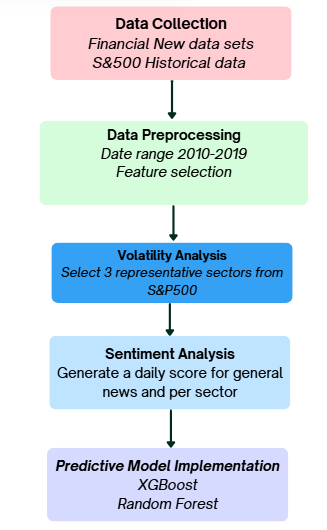
\includegraphics[width=\linewidth,height=0.78\textheight,keepaspectratio]{work_pipeline.png}
\end{center}

\column{0.36\textwidth}
\small
\heading{Four stages}
\begin{enumerate}
  \item Daily OHLCV from \texttt{yfinance} (2010--2019).
  \item Technical indicators \& target construction.
  \item Headline sentiment via FinBERT, aggregated by trading day.
  \item Tree ensembles: RF and XGBoost, with and without sentiment.
\end{enumerate}
\end{columns}
\end{frame}

% ------------------------------ Data sources ---------------------------------
\begin{frame}{Data sources}
\small
\begin{columns}[T,onlytextwidth]
\column{0.5\textwidth}
\heading{Historical market data}
\begin{itemize}
  \item Source: \texttt{yfinance} (Python wrapper of Yahoo Finance).
  \item Period: \textbf{Jan 2010 -- Dec 2019} \\(avoids COVID distortions and matches news coverage).
  \item Universe: S\&P 500 index (\texttt{\textasciicircum GSPC}) + the 11 GICS sector ETFs (\texttt{XLK},\texttt{XLV},\texttt{XLF},\dots).
  \item Variables: Open, High, Low, Close, Volume.
\end{itemize}

\column{0.5\textwidth}
\heading{Financial news}
\begin{itemize}
  \item Source: Kaggle ``Analyst Ratings Processed'' (\textgreater 1.4M headlines, 6,000+ tickers).
  \item Schema: \texttt{date}, \texttt{title}, \texttt{stock}.
  \item Filtered to S\&P 500 tickers and the 2010--2019 window.
  \item Stratified sample of \textbf{50 headlines / day} (\texttt{random\_state=42}) to bound FinBERT inference time.
\end{itemize}
\end{columns}

\vspace{6pt}
\begin{block}{Validation}
\small Missing OHLCV rows dropped, duplicates removed, dates aligned to trading calendar, news on non-trading days carried forward, neutral (0) sentiment imputed when no headlines are available for a day.
\end{block}
\end{frame}

% ------------------------------ Technical indicators -------------------------
\begin{frame}{Technical indicators}
\small
Seven indicators derived from OHLCV. All persisted to per-dataset CSVs in \texttt{datasets\_/}.

\vspace{6pt}
\begin{center}
\renewcommand{\arraystretch}{1.15}
\begin{tabular}{@{}l l l@{}}
\toprule
\textbf{Indicator} & \textbf{Definition} & \textbf{Role} \\
\midrule
\texttt{Returns}    & $r_t = (C_t - C_{t-1})/C_{t-1}$ & Momentum \\
\texttt{SMA\_10}    & 10-day simple moving average of $C_t$ & Trend \\
\texttt{EMA\_10}    & 10-day exponential moving average of $C_t$ & Trend (reactive) \\
\texttt{RSI}        & 14-period Wilder's relative-strength index & Overbought / oversold \\
\texttt{Volatility} & 10-day rolling standard deviation of $r_t$ & Risk \\
\texttt{HLC3}       & $(H_t+L_t+C_t)/3$ (typical price) & Price proxy \\
\texttt{Volume}     & Raw daily trading volume & Activity \\
\bottomrule
\end{tabular}
\end{center}

\vspace{6pt}
\heading{Target.} $y_t = \mathbf{1}\{C_{t+1} > C_t\}$ --- computed once at the data-preparation stage, before any modelling.
\end{frame}

% ------------------------------ Sector volatility ----------------------------
\begin{frame}{Volatility-based sector selection (2010--2019)}
\small Annualised volatility $\sigma = \mathrm{std}(r_t)\cdot\sqrt{252}$ for the 11 GICS sector ETFs.
The three highlighted sectors define the low / median / high-volatility datasets.

\vspace{2pt}
\begin{center}
  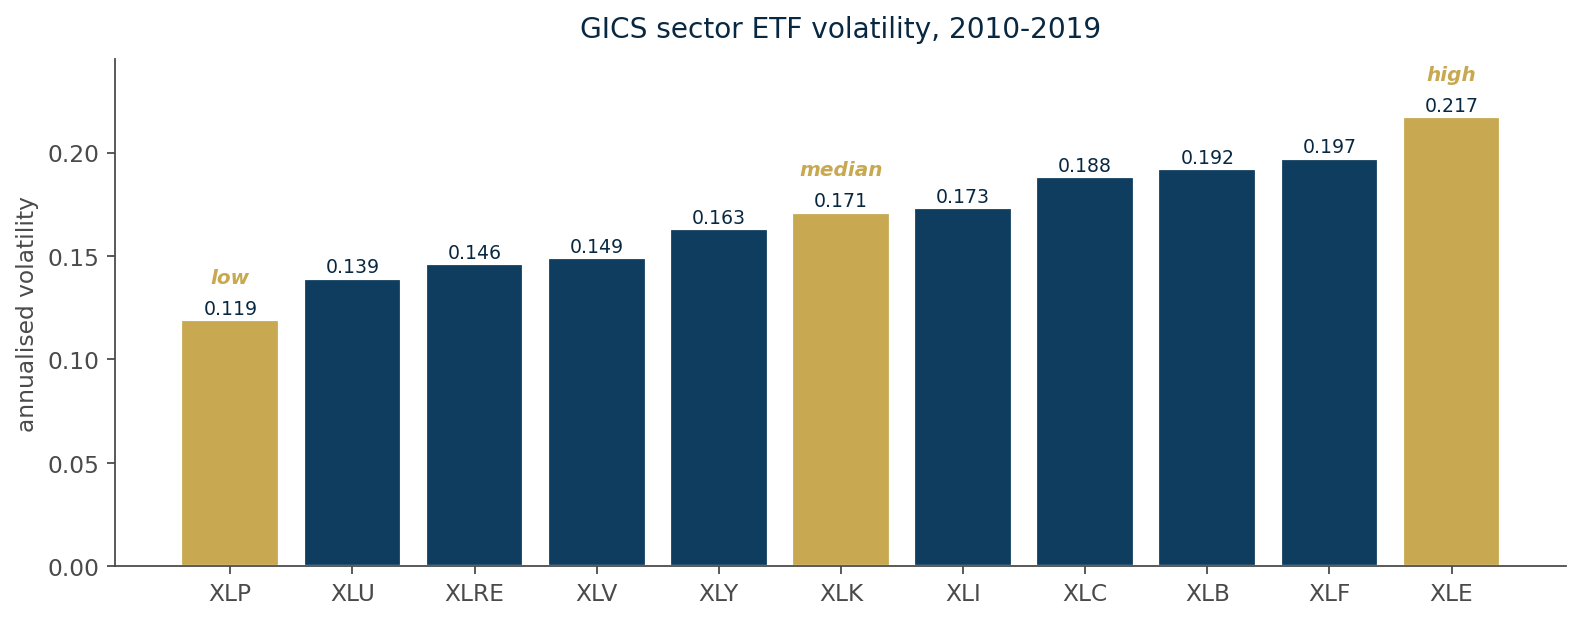
\includegraphics[width=0.98\linewidth,height=0.70\textheight,keepaspectratio]{sector_volatility.png}
\end{center}

\vspace{-4pt}
\centering\footnotesize
\textbf{XLP} (Consumer Staples) low \quad\textcolor{TecGold}{$\bullet$}\quad
\textbf{XLK} (Technology) median \quad\textcolor{TecGold}{$\bullet$}\quad
\textbf{XLE} (Energy) high
\end{frame}

% ------------------------------ FinBERT --------------------------------------
\begin{frame}{Sentiment pipeline --- FinBERT}
\begin{columns}[T,onlytextwidth]
\column{0.50\textwidth}
\begin{center}
  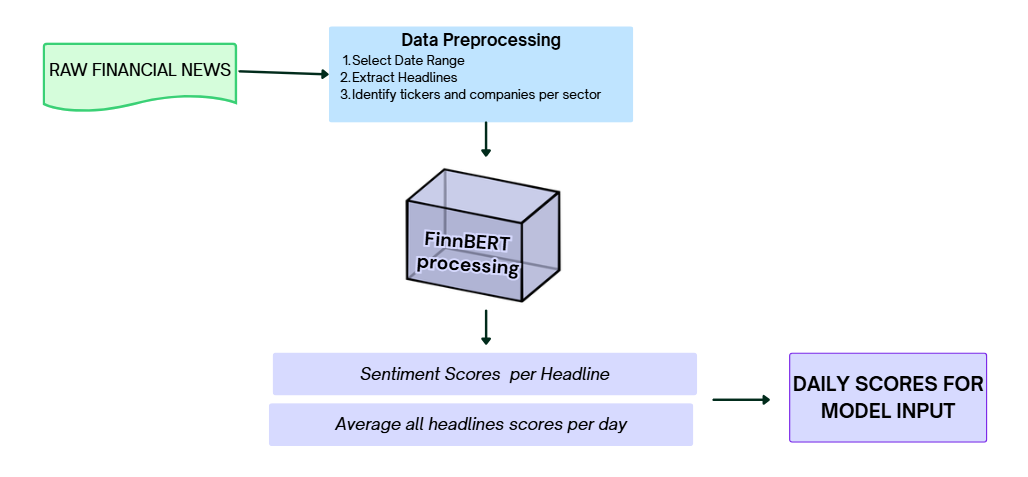
\includegraphics[width=\linewidth,height=0.72\textheight,keepaspectratio]{finbert_workflow.png}
\end{center}

\column{0.48\textwidth}
\small
\heading{Per headline}\\
\quad $s_i = P(\text{positive}_i) - P(\text{negative}_i),\ s_i\in[-1,1]$

\vspace{6pt}
\heading{Per trading day}
$$S_t \;=\; \frac{1}{n_t}\sum_{i=1}^{n_t} s_i$$
$$\sigma^{S}_t \;=\; \mathrm{std}(s_i),\quad N_t \;=\; n_t$$

\vspace{4pt}
\heading{Implementation}
\begin{itemize}
  \item \texttt{ProsusAI/finbert} via Hugging Face pipeline.
  \item Batch size 32, weighted score = sign of label $\times$ confidence.
  \item Days without headlines $\rightarrow$ neutral ($S_t=0$).
\end{itemize}
\end{columns}
\end{frame}

% ------------------------------ EDA: class balance -------------------------
\begin{frame}{EDA --- target class balance}
\begin{center}
  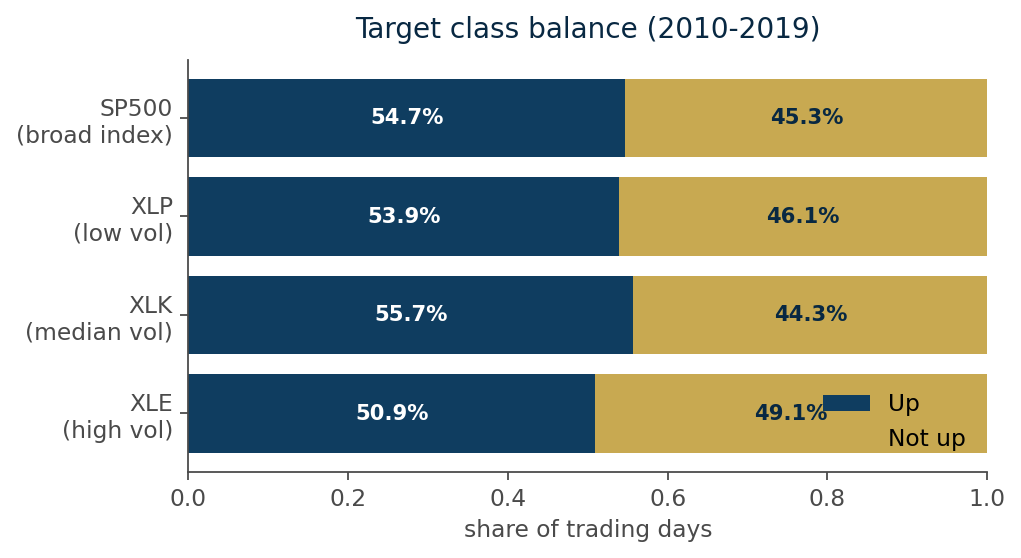
\includegraphics[width=0.92\linewidth,height=0.66\textheight,keepaspectratio]{class_balance.png}
\end{center}
\vspace{2pt}
\centering\footnotesize
Mild but consistent up-bias: a naive ``always-up'' baseline already scores $\approx 0.55$ accuracy.\\
AUC therefore remains the unbiased metric for ranking quality.
\end{frame}

% ------------------------------ EDA: news + sentiment -----------------------
\begin{frame}{EDA --- news flow and FinBERT sentiment distribution}
\begin{center}
  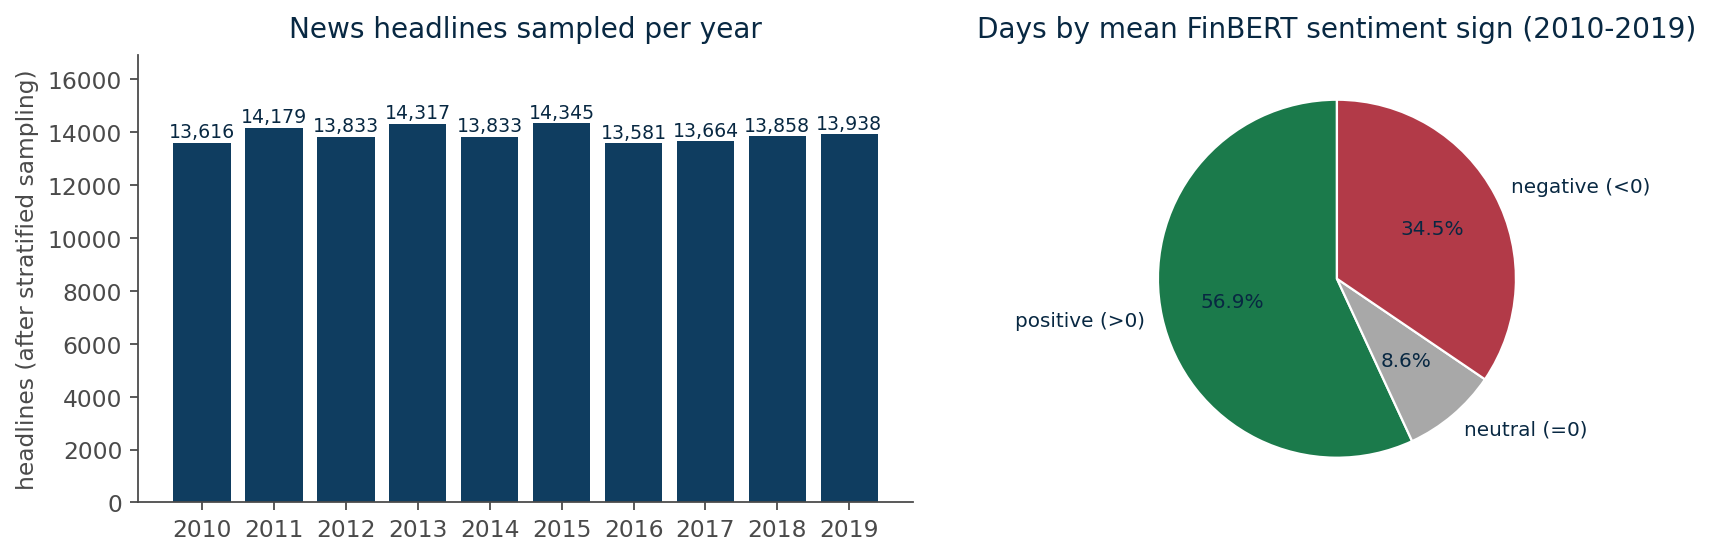
\includegraphics[width=0.98\linewidth,height=0.68\textheight,keepaspectratio]{eda_news_sentiment.png}
\end{center}
\vspace{-2pt}
\centering\footnotesize
$\sim$386K headlines scored over the 10-year window (stratified sample of up to 50 per day, \texttt{random\_state=42}).\\
Mean daily sentiment is mildly positive (+0.033, $\sigma=$0.168) --- coverage hits 100\% of trading days.
\end{frame}

% ------------------------------ Experimental design --------------------------
\begin{frame}{Experimental design}
\begin{columns}[T,onlytextwidth]
\column{0.6\textwidth}
\begin{center}
  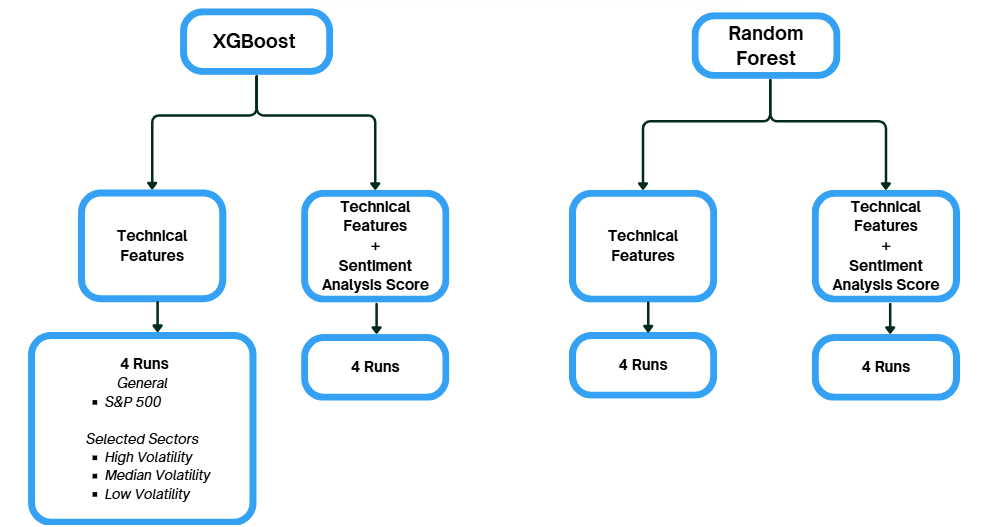
\includegraphics[width=\linewidth,height=0.7\textheight,keepaspectratio]{experimental_design.png}
\end{center}

\column{0.38\textwidth}
\small
\heading{Two algorithms}
\begin{itemize}
  \item Random Forest (\texttt{sklearn}).
  \item XGBoost.
\end{itemize}

\heading{Two feature sets}
\begin{itemize}
  \item Technical only (7 features).
  \item Technical + \texttt{sentiment\_mean} (8 features).
\end{itemize}

\heading{Four datasets}
\begin{itemize}
  \item SP500 broad index.
  \item XLP (low), XLK (median), XLE (high) sector ETFs.
\end{itemize}

\vspace{4pt}
$\Rightarrow$ \textbf{16 experimental runs.}
\end{columns}
\end{frame}

% ------------------------------ Train / metrics ------------------------------
\begin{frame}{Training protocol and evaluation}
\small
\begin{columns}[T,onlytextwidth]
\column{0.5\textwidth}
\heading{Chronological 80/20 split}
\begin{itemize}
  \item No shuffling --- prevents look-ahead bias.
  \item For each dataset: $\approx$ 2{,}000 train days / 501 test days.
  \item Same split for every algorithm and feature configuration.
\end{itemize}

\heading{Hyper-parameters}
\begin{itemize}\setlength\itemsep{2pt}
  \item RF: \texttt{n\_estimators=100}, default depth, \texttt{random\_state=42}.
  \item XGB: \texttt{n\_estimators=100}, default depth, \texttt{eval\_metric="logloss"}, \texttt{random\_state=42}.
\end{itemize}

\column{0.5\textwidth}
\heading{Metrics}
\begin{itemize}
  \item \textbf{Accuracy} --- overall correctness.
  \item \textbf{F1-score} --- harmonic mean of precision/recall, robust to class imbalance.
  \item \textbf{AUC-ROC} --- threshold-free ranking quality.
\end{itemize}

\heading{Why all three}
A trivial ``always up'' classifier can score $\sim$0.55 accuracy and $\sim$0.70 F1 yet have AUC $\approx$ 0.50. Reporting AUC alongside Accuracy/F1 prevents false confidence.
\end{columns}
\end{frame}

% ------------------------------ Results: technical ---------------------------
\begin{frame}{Results --- technical features only}
\begin{center}
  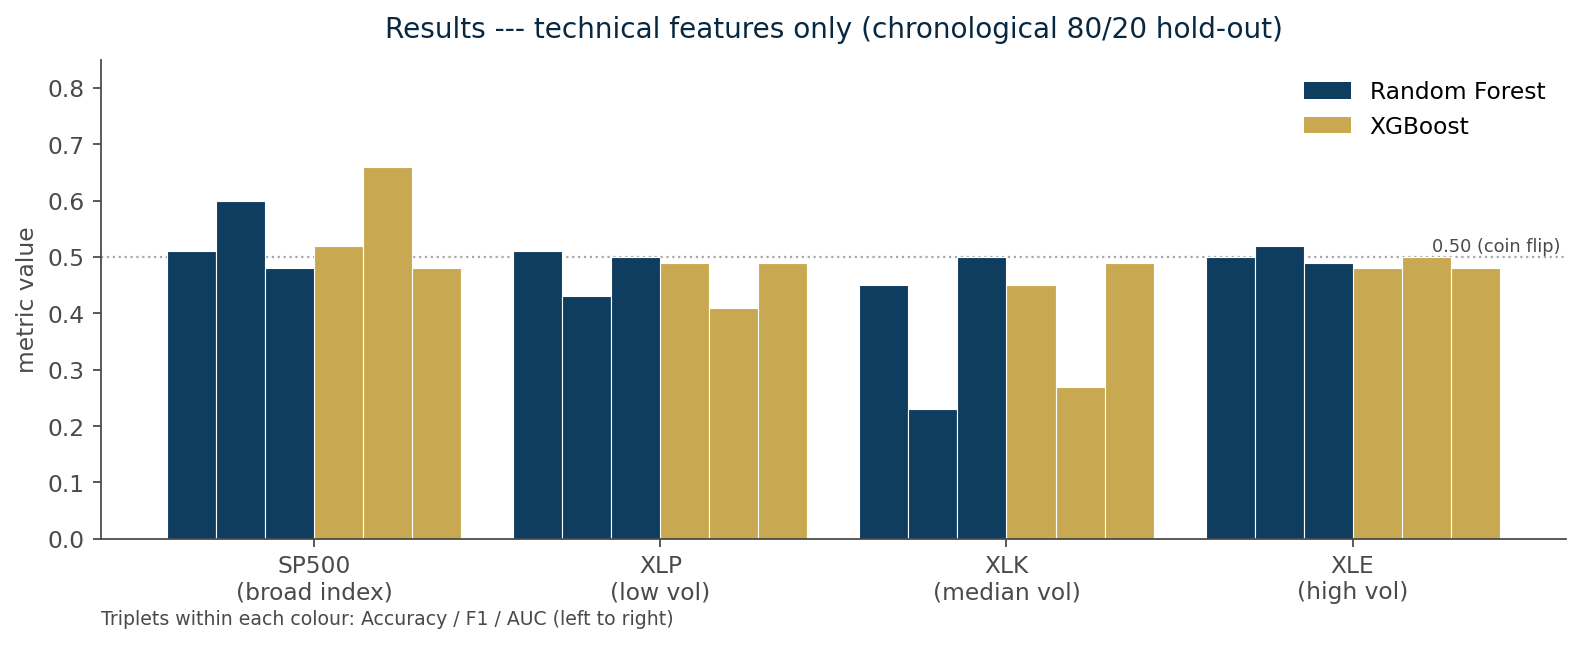
\includegraphics[width=0.98\linewidth,height=0.72\textheight,keepaspectratio]{results_technical_only.png}
\end{center}
\vspace{-4pt}
\centering\footnotesize
AUC clusters around 0.50 $\Rightarrow$ technical features alone barely separate up from non-up days.
XGB on SP500 reaches F1 = 0.66 only because it leans on the majority class.\\
\textbf{XLK} collapses to class 0 in this window (F1 = 0.23 / 0.27).
\end{frame}

% ------------------------------ Results: sentiment ---------------------------
\begin{frame}{Results --- technical + FinBERT sentiment}
\begin{center}
  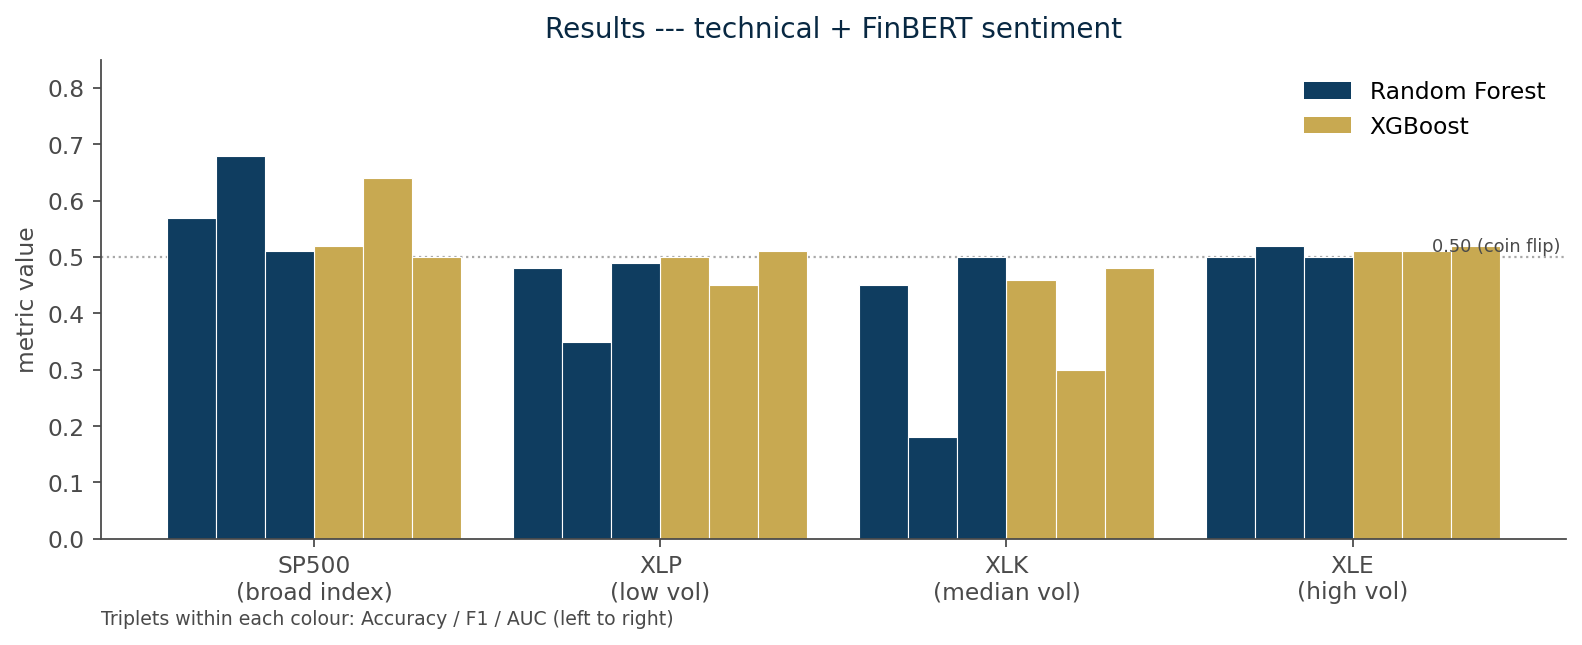
\includegraphics[width=0.98\linewidth,height=0.72\textheight,keepaspectratio]{results_technical_sentiment.png}
\end{center}
\vspace{-4pt}
\centering\footnotesize
\good{SP500 + RF + sentiment} jumps to \textbf{0.57 Acc / 0.68 F1 / 0.51 AUC} (+0.06 / +0.08 / +0.04). \\
\good{XLE + XGB + sentiment} pushes AUC from 0.48 to 0.52 ---
sentiment moves the needle on the broad index and on the high-volatility sector only.
\end{frame}

% ------------------------------ Delta plot -----------------------------------
\begin{frame}{Sentiment uplift at a glance}
\begin{center}
  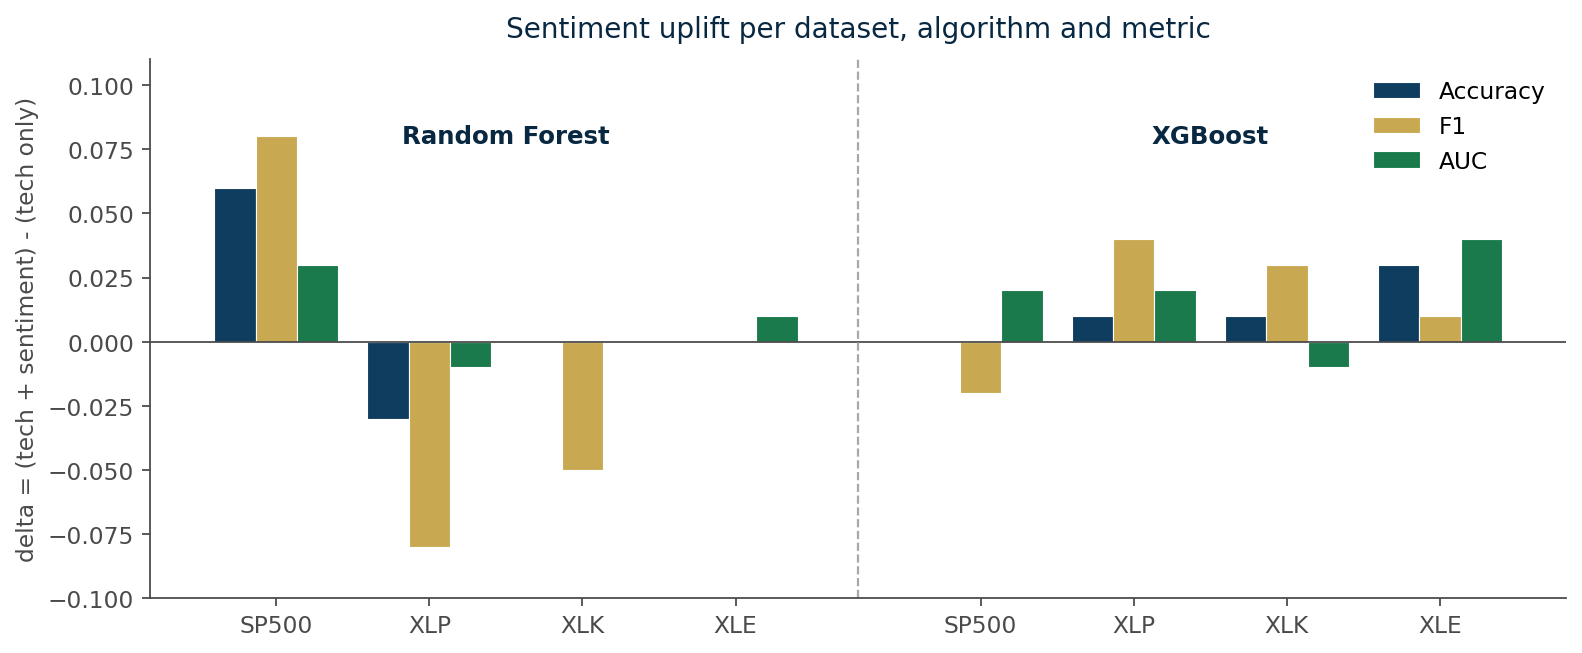
\includegraphics[width=0.98\linewidth,height=0.74\textheight,keepaspectratio]{sentiment_uplift.png}
\end{center}
\vspace{-2pt}
\centering\footnotesize
Strongest positive cluster: \good{SP500 + RF} (all three metrics) and \good{XLE + XGB} (Acc and AUC).
\textbf{XLP under RF} is the only configuration where sentiment hurts on every metric.
\end{frame}

% ------------------------------ Feature importance ---------------------------
\begin{frame}{Where does the signal come from? Feature importance}
\begin{center}
  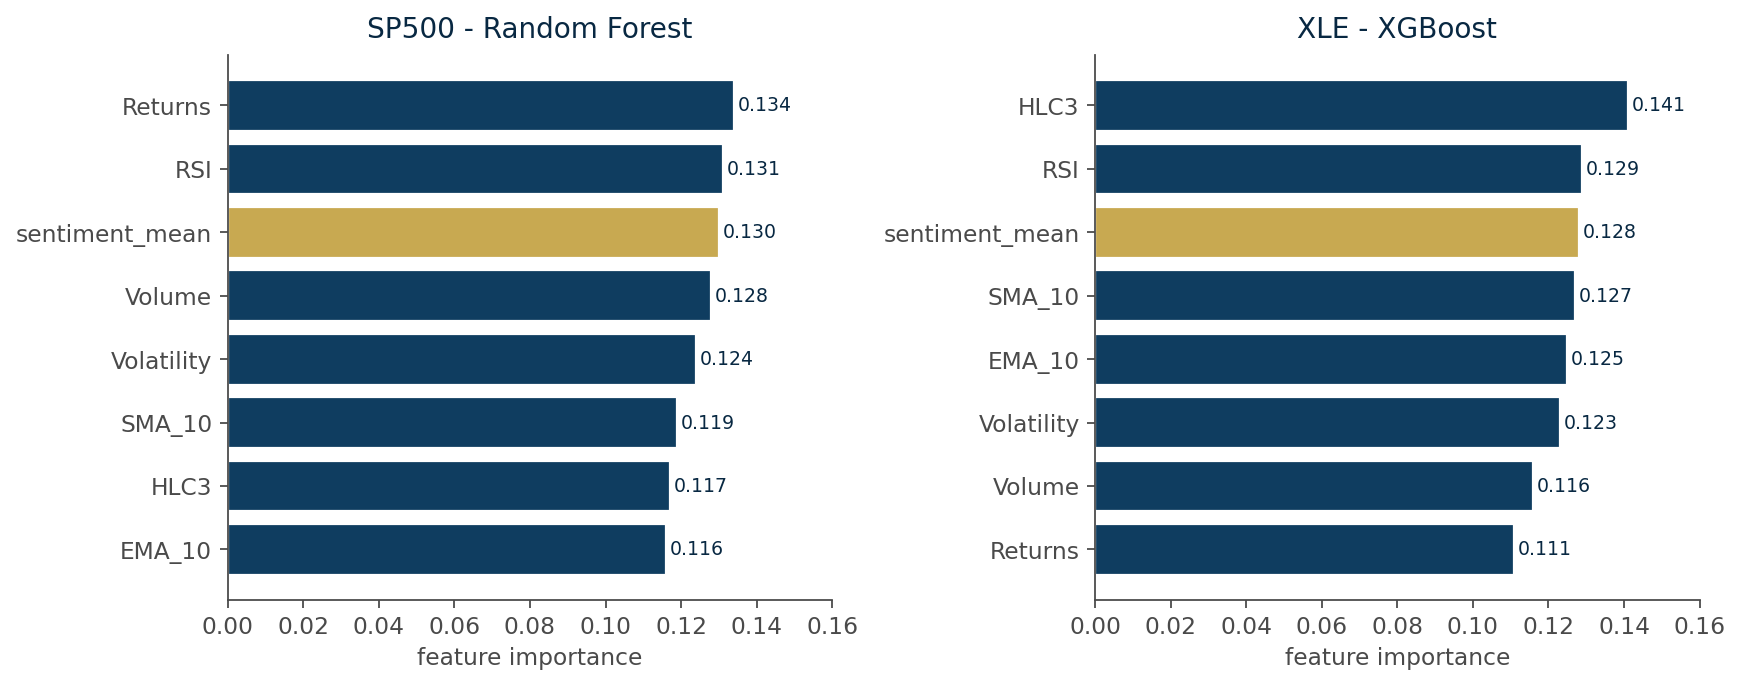
\includegraphics[width=0.98\linewidth,height=0.74\textheight,keepaspectratio]{feature_importance.png}
\end{center}
\vspace{-2pt}
\centering\footnotesize
\textbf{sentiment\_mean} (gold) ranks in the \textbf{top three} for the two configurations where it materially improved AUC.\\
Tree ensembles spread importance fairly evenly across the seven technical features --- no single indicator dominates.
\end{frame}

% ------------------------------ Hypothesis check -----------------------------
\begin{frame}{Hypothesis assessment}
\small
\begin{block}{H1 --- ``Sentiment improves prediction.''}
\textit{Partially supported.} The broad SP500 index sees a meaningful Random Forest improvement on all three metrics. Sector-level effects are inconsistent: XLE benefits, XLP and XLK do not.
\end{block}

\begin{block}{H2 --- ``Higher volatility $\Rightarrow$ larger sentiment gain.''}
\textit{Partially supported.} XLE (highest vol) shows the largest positive XGB delta. However, XLK (median vol) does not benefit, so the volatility$\rightarrow$benefit gradient is not monotonic.
\end{block}

\begin{block}{RQ2 --- ``Random Forest or XGBoost?''}
On AUC the two algorithms are tied. \textbf{Random Forest} wins on the SP500 index when sentiment is included; \textbf{XGBoost} wins on the high-volatility XLE sector.
\end{block}
\end{frame}

% ------------------------------ Live demo -----------------------------------
\begin{frame}{Live demo --- predict tomorrow on Google Colab}
\small A recorded walk-through of the companion Colab notebook running the four pre-trained classifiers on a \textbf{fully live} pipeline: today's OHLCV from Yahoo Finance, today's headlines scored with FinBERT, and the next-day \textbf{UP} / \textbf{DOWN} / \textbf{STABLE} call printed for each model.

\vspace{8pt}
\begin{columns}[T,onlytextwidth]
\column{0.58\textwidth}
\heading{What the notebook does (end-to-end)}
\begin{enumerate}\setlength\itemsep{2pt}
  \item Loads the four pre-trained classifiers (\texttt{rf\_tech}, \texttt{rf\_all}, \texttt{xgb\_tech}, \texttt{xgb\_all}) from \texttt{models\_demo/} on GitHub.
  \item Pulls today's OHLCV bar from \texttt{yfinance} and rebuilds the seven technical indicators in real time.
  \item Fetches today's Yahoo Finance headlines, scores them with \texttt{ProsusAI/finbert}, and aggregates a daily \texttt{sentiment\_mean} --- the same logic as Notebook 05.
  \item Feeds the live vector to all four models and maps $P(\text{up})$ to a label via the 0.45 / 0.55 thresholds.
\end{enumerate}

\column{0.42\textwidth}
\begin{block}{Watch the demo}
\centering
\href{https://drive.google.com/file/d/1WS7XSWKpDwQto0w0laguOEvEsgL1kAas/view?usp=sharing}{\textbf{\color{TecBlue}Recorded walk-through} \,\textcolor{TecGold}{$\rightarrow$}\, click here} \\[6pt]
\scriptsize \texttt{notebooks/08\_demo\_next\_day\_prediction.ipynb}
\end{block}

\vspace{4pt}
\heading{Source repository}\\
\scriptsize \texttt{github.com/brendangelica/}\\\texttt{sp500-predictor-}

\vspace{4pt}
\heading{Optional}\\
\scriptsize Override \texttt{TODAY\_SENTIMENT} to run a what-if scenario in $[-1,1]$.
\end{columns}

\vspace{4pt}
\centering\footnotesize\textit{Probabilities inside $[0.45, 0.55]$ are interpreted as ``stable / uncertain''.}
\end{frame}

% ------------------------------ Discussion -----------------------------------
\begin{frame}{Discussion}
\small
\begin{itemize}
  \item \heading{AUC near 0.50.} Consistent with the weak form of the Efficient Market Hypothesis --- price-only signals offer at most a marginal next-day edge.
  \item \heading{Sentiment is a thin signal at this granularity.} Daily-aggregated headline sentiment loses intra-day timing; the noisiest sectors mask its contribution.
  \item \heading{Class collapse on XLK.} The 2018--2019 test window contained more flat / down days than up days; without class re-weighting the model takes the easy way out.
  \item \heading{Why SP500 benefits the most.} Index-level returns aggregate idiosyncratic noise, leaving systematic news flow as a relatively cleaner signal.
\end{itemize}
\end{frame}

% ------------------------------ Limitations ----------------------------------
\begin{frame}{Limitations}
\small
\begin{itemize}
  \item \heading{News coverage skew.} The Kaggle headline corpus emphasises U.S.-listed mega-caps; smaller sector constituents are under-represented.
  \item \heading{Headline-only sentiment.} Body text and analyst-report tone are ignored; FinBERT operates on short titles only.
  \item \heading{Sampling cap.} Up to 50 headlines per day is a compute-driven compromise --- bullish news clusters may be undercounted on heavy-news days.
  \item \heading{Single train / test cut.} A walk-forward backtest would offer stronger evidence than one 80/20 chronological split.
  \item \heading{Hyper-parameters not tuned.} Defaults are used to keep all 16 runs directly comparable.
\end{itemize}
\end{frame}

% ------------------------------ Conclusions ----------------------------------
\begin{frame}{Conclusions}
\small
\begin{block}{Take-aways}
\begin{enumerate}
  \item Headline sentiment from FinBERT \alert{helps at the index level} when paired with Random Forest: +0.06 Acc, +0.08 F1, +0.04 AUC over the technical-only baseline.
  \item The sentiment effect is \alert{not monotonic in sector volatility}: high-vol XLE benefits, low-vol XLP does not, but median-vol XLK also fails to benefit.
  \item Tree ensembles alone cannot break the AUC $\approx$ 0.50 ceiling on individual sectors --- a finding aligned with EMH-style expectations.
\end{enumerate}
\end{block}
\end{frame}

% ------------------------------ Future work ----------------------------------
\begin{frame}{Future work}
\small
\begin{itemize}
  \item \heading{Walk-forward evaluation} with expanding training windows.
  \item \heading{Multi-resolution sentiment}: pair daily aggregates with $K$-day moving averages and event-time deltas.
  \item \heading{Sector-aware news routing}: weight headlines by the ticker's sector weight to better align signal with target.
  \item \heading{Class re-weighting or stratification} to fix XLK's collapse onto the majority class.
  \item \heading{Calibrated thresholds} to make AUC gains actionable in a trading-signal context.
  \item \heading{Out-of-sample 2020--2024 stress test} once a COVID-normalisation feature is added.
\end{itemize}
\end{frame}

% ------------------------------ References -----------------------------------
\begin{frame}[allowframebreaks]{Selected references}
\small
\begin{thebibliography}{99}
\bibitem{bollen2011} J. Bollen, H. Mao, X. Zeng. ``Twitter mood predicts the stock market.'' \textit{J.\ Computational Science}, 2(1):1--8, 2011.
\bibitem{vargas2017} M.\ R.\ Vargas et al. ``Deep learning for stock market prediction from financial news.'' \textit{IEEE CIVEMSA}, 2017.
\bibitem{araci2019}  D. Araci. ``FinBERT: Financial Sentiment Analysis with Pre-trained Language Models.'' arXiv:1908.10063, 2019.
\bibitem{zhang2019} B. Zhang, J. Huang, J. Zhou. ``Stock price prediction via XGBoost.'' \textit{IEEE Big Data}, 2019.
\bibitem{prado2018}  M. L\'opez de Prado. \textit{Advances in Financial Machine Learning}. Wiley, 2018.
\bibitem{breiman2001} L. Breiman. ``Random Forests.'' \textit{Machine Learning} 45(1):5--32, 2001.
\bibitem{chen2016} T. Chen, C. Guestrin. ``XGBoost: A Scalable Tree Boosting System.'' \textit{ACM KDD}, 2016.
\bibitem{fama1970} E. F. Fama. ``Efficient capital markets.'' \textit{J.\ Finance}, 25(2):383--417, 1970.
\bibitem{mostafavi2025} S. M. Mostafavi, A. R. Hooman. ``Key technical indicators for stock market prediction.'' \textit{Machine Learning with Applications}, 20:100631, 2025.
\end{thebibliography}
\end{frame}

% ------------------------------ Thanks ---------------------------------------
{
\setbeamertemplate{footline}{}
\begin{frame}[plain]
\begin{tikzpicture}[remember picture,overlay]
  \fill[TecBlue]     (current page.north west) rectangle (current page.south east);
  \fill[TecGold]     ([yshift=-2.4cm]current page.north west) rectangle ([yshift=-2.48cm]current page.north east);
  \node[anchor=center,white] at (current page.center) {%
    \begin{minipage}{0.85\paperwidth}\centering
      {\fontsize{30}{34}\selectfont\textbf{Thank you.}}\\[14pt]
      {\fontsize{16}{20}\selectfont\textit{Questions and discussion}}\\[28pt]
      {\fontsize{11}{14}\selectfont
        C\'esar Emilio Casta\~no Mar\'in \,\textcolor{TecGold}{$\bullet$}\, A00830006 \\
        Brenda Ang\'elica Garc\'ia \,\textcolor{TecGold}{$\bullet$}\, A01633622 \\[6pt]
        \textit{Tecnol\'ogico de Monterrey --- Data Analytics --- M.Sc. CS}}
    \end{minipage}};
\end{tikzpicture}
\end{frame}
}

% ------------------------------ Appendix -------------------------------------
\appendix

\begin{frame}{Appendix --- Acronyms}
\small
\begin{columns}[T,onlytextwidth]
\column{0.50\textwidth}
\renewcommand{\arraystretch}{1.25}
\begin{tabular}{@{}l l@{}}
\textbf{AUC}    & Area Under the (ROC) Curve \\
\textbf{BERT}   & Bidirectional Encoder Representations \\
                & from Transformers \\
\textbf{CNN}    & Convolutional Neural Network \\
\textbf{EMA}    & Exponential Moving Average \\
\textbf{EMH}    & Efficient Market Hypothesis \\
\textbf{ETF}    & Exchange-Traded Fund \\
\textbf{F1}     & F1 score (harmonic mean of P and R) \\
\textbf{FinBERT}& Finance-domain BERT (Araci 2019) \\
\textbf{GICS}   & Global Industry Classification Std. \\
\textbf{HLC3}   & (High + Low + Close) / 3 \\
\textbf{ML}     & Machine Learning \\
\textbf{NLP}    & Natural Language Processing \\
\end{tabular}

\column{0.50\textwidth}
\renewcommand{\arraystretch}{1.25}
\begin{tabular}{@{}l l@{}}
\textbf{OHLCV}  & Open, High, Low, Close, Volume \\
\textbf{P / R}  & Precision / Recall \\
\textbf{RF}     & Random Forest \\
\textbf{RNN}    & Recurrent Neural Network \\
\textbf{ROC}    & Receiver Operating Characteristic \\
\textbf{RQ}     & Research Question \\
\textbf{RSI}    & Relative Strength Index \\
\textbf{S\&P 500} & Standard \& Poor's 500 index \\
\textbf{SMA}    & Simple Moving Average \\
\textbf{TP / TN}& True Positive / True Negative \\
\textbf{FP / FN}& False Positive / False Negative \\
\textbf{XGB / XGBoost} & Extreme Gradient Boosting \\
\textbf{\^{}GSPC} & Yahoo Finance ticker for S\&P 500 \\
\end{tabular}
\end{columns}
\end{frame}

\begin{frame}{Appendix --- Glossary (1/2): finance and indicators}
\small
\renewcommand{\arraystretch}{1.25}
\begin{tabular}{@{}p{3.2cm} p{11cm}@{}}
\heading{S\&P 500 index} & Capitalisation-weighted index tracking 500 of the largest U.S. publicly traded companies; benchmark for U.S. equity market health. \\
\heading{GICS sector} & One of eleven Global Industry Classification Standard groupings (Tech, Financials, Energy, etc.) used to partition the S\&P 500 into thematic sub-universes. \\
\heading{Sector ETF} & Exchange-traded fund that replicates the performance of a GICS sector --- e.g.\ \texttt{XLP} (Consumer Staples), \texttt{XLK} (Technology), \texttt{XLE} (Energy). \\
\heading{OHLCV} & The five raw daily bars from Yahoo Finance: \textbf{O}pen, \textbf{H}igh, \textbf{L}ow, \textbf{C}lose, \textbf{V}olume. \\
\heading{Daily return} & Percentage change in closing price between two consecutive trading days, $r_t = (C_t - C_{t-1})/C_{t-1}$. \\
\heading{Volatility} & In this work, the 20-day rolling standard deviation of daily returns; annualised by multiplying by $\sqrt{252}$. \\
\heading{HLC3 (typical price)} & $(H_t + L_t + C_t)/3$. Robust proxy of the day's traded price. \\
\heading{SMA / EMA} & Simple / Exponential moving averages of the closing price over a window of 10 days. EMA reacts faster to recent moves. \\
\heading{RSI} & Wilder's 14-period Relative Strength Index; bounded in $[0,100]$. Conventional thresholds: $>70$ overbought, $<30$ oversold. \\
\heading{EMH} & Efficient Market Hypothesis (Fama, 1970): prices already reflect all available information, so consistent prediction is hard. \\
\end{tabular}
\end{frame}

\begin{frame}{Appendix --- Glossary (2/2): NLP and machine learning}
\small
\renewcommand{\arraystretch}{1.25}
\begin{tabular}{@{}p{3.2cm} p{11cm}@{}}
\heading{FinBERT} & BERT language model fine-tuned by Araci (2019) on a corpus of financial text; returns probabilities of \textit{positive}, \textit{negative}, and \textit{neutral} sentiment for a given input string. \\
\heading{Sentiment score} & Net per-headline score $s_i = P(\text{pos}) - P(\text{neg}) \in [-1, 1]$, aggregated per trading day as a confidence-weighted mean. \\
\heading{Target $y_t$} & Binary label: $1$ if $C_{t+1} > C_t$, else $0$. We predict \textit{direction}, not price. \\
\heading{Random Forest} & Bagging ensemble of decision trees, each trained on a bootstrap sample with random feature subsets; majority vote for prediction (Breiman 2001). \\
\heading{XGBoost} & Gradient-boosted trees with regularisation; trees built sequentially to correct residuals of the running ensemble (Chen \& Guestrin 2016). \\
\heading{Chronological split} & Train on the first 80\% of trading days and test on the last 20\%, never shuffling --- prevents look-ahead bias. \\
\heading{Accuracy} & $(TP + TN) / (TP + TN + FP + FN)$. \\
\heading{Precision / Recall} & $P = TP/(TP+FP)$; $R = TP/(TP+FN)$. \\
\heading{F1 score} & Harmonic mean of precision and recall: $F_1 = 2PR / (P+R)$. \\
\heading{AUC-ROC} & Area under the Receiver Operating Characteristic curve; threshold-free measure of ranking quality. $0.5$ = random, $1.0$ = perfect. \\
\heading{Look-ahead bias} & Using information unavailable at prediction time; avoided by chronological splits and lagged feature engineering. \\
\end{tabular}
\end{frame}

\begin{frame}{Appendix --- Improvement variant explored}
\small Adds \texttt{sentiment\_std} and \texttt{news\_volume}; RF 300/depth=12 with class-balanced weights; XGB 300/depth=6/lr=0.05.

\vspace{4pt}
\begin{center}
\renewcommand{\arraystretch}{1.15}
\begin{tabular}{@{}l l c c c c c c@{}}
\toprule
\textbf{Dataset} & \textbf{Feat.\ set} & \textbf{RF Acc} & \textbf{RF F1} & \textbf{RF AUC} & \textbf{XGB Acc} & \textbf{XGB F1} & \textbf{XGB AUC} \\
\midrule
SP500 & Tech.        & 0.54 & 0.69 & 0.47 & 0.55 & 0.69 & 0.50 \\
SP500 & Tech.+Sent.  & 0.54 & 0.68 & 0.48 & 0.54 & 0.68 & 0.49 \\
XLE   & Tech.        & 0.49 & 0.50 & 0.49 & 0.49 & 0.52 & 0.50 \\
XLE   & Tech.+Sent.  & \textbf{0.52} & \textbf{0.53} & \textbf{0.51} & \textbf{0.54} & \textbf{0.57} & \textbf{0.52} \\
\bottomrule
\end{tabular}
\end{center}

\vspace{4pt}
\textbf{Takeaway.} Adds \textit{some} stability for the highest-vol sector but does not break the AUC $\approx$ 0.50 ceiling; conclusions of the main study hold.
\end{frame}

\begin{frame}{Appendix --- Detailed metric definitions}
\small
\heading{Confusion-matrix counts.} TP, TN, FP, FN are computed on the chronological 20\% test set.

\vspace{4pt}
\begin{center}
\renewcommand{\arraystretch}{1.25}
\begin{tabular}{@{}l l l@{}}
\toprule
\textbf{Metric} & \textbf{Formula} & \textbf{Reading} \\
\midrule
Accuracy   & $\dfrac{TP+TN}{TP+TN+FP+FN}$                          & overall correctness, threshold-dependent \\
Precision  & $\dfrac{TP}{TP+FP}$                                   & of the predicted up days, how many were right \\
Recall     & $\dfrac{TP}{TP+FN}$                                   & of the actual up days, how many we caught \\
F1-score   & $\dfrac{2\,P\,R}{P+R}$                                & harmonic mean of P and R \\
AUC-ROC    & $\int_0^1 \mathrm{TPR}(\mathrm{FPR}^{-1}(u))\, du$    & threshold-free ranking quality \\
\bottomrule
\end{tabular}
\end{center}

\vspace{6pt}
\heading{Why all three.} A naive ``always-up'' classifier on SP500 (54.7\% up days) gets Accuracy 0.55 and F1 $\approx$ 0.71 but AUC = 0.50.
\end{frame}

\end{document}
